%% UH Manoa thesis class (https://github.com/rbrewer/latex-uhm-thesis).
%% uhthesis.cls sits next to this file. Class defaults: 11pt, letter paper,
%% one-sided, 1.5 spacing, master's thesis. Add "draft" for single-spaced
%% drafts that print today's date and \versionnum on the title page.
\documentclass[11pt]{uhthesis}

\usepackage{cite}
\usepackage{mathtools}
\usepackage{amsthm,amsmath,amssymb,amsfonts}
\usepackage{algorithmic}
\usepackage{graphicx}
\usepackage{textcomp}
\usepackage{url}
%\usepackage{todonotes}
\usepackage[disable]{todonotes}
\usepackage{paralist}
\usepackage{hyperref}
\usepackage{tikz}
\usepackage{enumitem}
\usetikzlibrary{positioning,arrows.meta,calc}

\usepackage{xspace}
\usepackage{xcolor}


\newcommand{\HC}[2][inline]{\todo[color=blue!50,#1]{\sf \small\textbf{HC:} #2\normalsize}\xspace}
\newcommand{\VP}[2][inline]{\todo[color=green!50,#1]{\sf \small\textbf{VP:} #2\normalsize}\xspace}
\newcommand{\FS}[2][inline]{\todo[color=yellow!50,#1]{\sf \small\textbf{FS:} #2\normalsize}\xspace}
\newcommand{\TODO}[2][inline]{\todo[color=red!30,#1]{\sf \small\textbf{TODO:} #2\normalsize}\xspace}
\newcommand{\DONE}[2][inline]{\todo[color=green!30,#1]{\sf \small\textbf{DONE:} #2\normalsize}\xspace}

\newcommand{\efail}{\ensuremath{e_{f}}\xspace}
\newcommand{\N}{\mathbb{N}}
\newcommand{\Z}{\mathbb{Z}}
\newcommand{\R}{\mathbb{R}}
\newcommand{\deltat}{\ensuremath{\delta}\xspace}
\newcommand{\psuc}[1]{e^{-\lambda #1 \deltat}}
\newcommand{\knapsack}{\textsc{Knapsack}\xspace}
\newtheorem{proposition}{Proposition}

\newcommand{\dynamic}{\textsc{Dyn}\xspace}
\newcommand{\random}{\textsc{Rand}\xspace}
\newcommand{\foresighted}{\textsc{Fs}\xspace}
\newcommand{\nearsighted}{\textsc{Ns}\xspace}

\newcommand{\errorlevel}{\textsc{E}\xspace}
\newcommand{\probsuccess}{\textsc{P}\xspace}
\newcommand{\ratio}{\textsc{R}\xspace}
\newcommand{\expectederror}{\textsc{X}\xspace}

\newcommand{\independent}{\textsc{Ind}\xspace}
\newcommand{\dependent}{\textsc{Dep}\xspace}
\newcommand{\aggressive}{\textsc{Agg}\xspace}
\newcommand{\variant}{\textsc{Var}\xspace}
\newcommand{\off}{\textsc{Off}\xspace}

\newcommand{\strategy}[3]{{#1}/{#2}/{#3}}

%%% Front matter declarations. Capitalize normally; the class reformats them.

\title{Deadline-Constrained Scheduling of Multi-Mode Task Chains under Fail-Stop Failures}

% Real-Time Scheduling of Chains of Multi-Mode Tasks To under Fail-Stop Failures}
% Real-Time Scheduling of Chains of Approximate Computation Tasks in the Presence of Fail-Stop Errors
% Real-Time Scheduling of Chains of Multi-Mode Tasks To Minimize Expected Output Error under Fail-Stop Failures
% Real-Time Scheduling of Chains of Tasks with Multiple Execution Options to Minimize Expected Output Error under Fail-Stop Failures

%% No titles (Dr., Prof.) in any of the names below.
\author{Victor Pagan}
%% TODO: month (May, August, or December) and year the degree is conferred.
\degreemonth{May}
\degreeyear{2027}
\degree{Master of Science}
\field{Computer Science}
%% TODO: confirm the chairperson and list the other committee members,
%% separated by "\\" (outside member last).
\chair{Henri Casanova}
\othermembers{Committee Member Two\\
Committee Member Three}
\keywords{fault tolerance, deadline-constrained scheduling, multi-mode task chains}
%% Only printed on the title page with the "draft" or "proposal" class option.
\versionnum{0.1.0}

\begin{document}

%% The title page counts as page i (unnumbered); roman numbering here keeps
%% hyperref's page anchors distinct from page 1 of the body.
\pagenumbering{roman}
\maketitle

\begin{frontmatter}

%%% Optional front matter pages, in the order the class expects:
%\copyrightpage
%\begin{dedication} ... \end{dedication}
%\begin{acknowledgments} ... \end{acknowledgments}

\begin{abstract}
Scheduling real-time applications in the presence of failures is
challenging.  In many domains, some level of output error is tolerable:
application tasks offer different execution modes, where modes with longer
execution times lead to lower error.  This provides an opportunity for
meeting real-time constraints in the presence of failures by trading off
higher error for faster task executions.  In this context, we study the
problem of scheduling a chain of multi-mode tasks onto a failure-prone
platform, allowing for replication, rollback/recovery, adaptive mode
changes after failures, reuse of persistent intermediate outputs, and
coordination across multiple processing elements. The objective is to
minimize the expected error in the final output produced by a deadline,
with a penalty if no output is produced.  For the case in which the
platform comprises a single processing element, we develop a dynamic
program that computes optimal scheduling decisions for the time-discretized
problem under the assumption that a task is never re-executed after it has
successfully completed once.  We also show how to select an appropriate
discretization resolution in practice.  When the platform comprises
multiple processing elements, we propose various heuristics, several of
which build on the above dynamic program.  We demonstrate and/or evaluate
our dynamic programming approach and heuristics via simulated executions
for a fusion energy application derived from a production use case and for
a large set of synthetic workloads.

\end{abstract}

\tableofcontents

\listoftables

\listoffigures

\end{frontmatter}

\chapter{Introduction}
\label{sec:introduction}

%\HC{Perhaps cite~\cite{10.1002_cpe.8019} as another example of a real-time workflow? Not sure}

Executions on compute platforms are subject to hardware
and software errors. An active area of research is application scheduling
in the presence of failures in non-real-time~\cite{10.5555/2811302}
or real-time~\cite{10.1145/3589950} settings, typically using
rollback/recovery and/or computation replication techniques.  In this work, 
we focus on deadline-constrained scientific computing applications, which
are increasingly commonplace across the sciences (see a recent
U.S. Department of Energy study~\cite{IRI-workflows}).

In many domains, approximate computing techniques~\cite{10.1145/3716845}
make it possible to implement application tasks with multiple \emph{execution
modes}. Each mode corresponds to a trade-off between execution
time and output error, where an erroneous output retains some utility.
Trading off output quality for a
shorter execution time provides an opportunity to meet real-time deadlines
that would otherwise be missed, motivating the development of strategies
for scheduling approximate computing applications in the presence of
failures~\cite{10.1145/2442087.2442094, 10.1007/s11227-021-03764-x,
259428, 10.1177/0037549709340729, 10.1109/TC.2003.1183950, 7570524}.


In this work we consider an application structured as a chain of tasks,
some of which have multiple modes of execution. The application executes on
a platform comprised of one or more processing elements (PEs) and is
subject to fail-stop failures.  Given an end-to-end deadline, the objective
is to make scheduling decisions that minimize the expected error of the
best final output produced by that deadline, assigning a user-defined penalty
when no final output is produced.  Prior work~\cite{10678736}
considers static replication and resource provisioning in this setting. 
Instead, we consider dynamic scheduling decisions 
that can employ replication, rollback/recovery,
execution mode changes after failures, reuse of persistent intermediate
outputs, and coordinated scheduling across PEs.  Specifically, we make the
following contributions:
\begin{compactitem}
    \item We formulate the problem and show its NP-hardness;
    \item For one-PE platforms we discretize time to develop a dynamic programming approach, together with a practical method for selecting the discretization resolution;
    \item For multiple-PE platforms we propose heuristics, some of which build on our results for the one-PE case; and
    \item We evaluate our scheduling strategies in simulation, both for a production workload from the field of fusion energy science and for a large set of synthetic workloads. 
\end{compactitem}

The rest of this thesis is organized as follows. Chapter~\ref{sec:use-case}
details a production use case that motivates our scheduling problem, which
is formalized in Chapter~\ref{sec:problem}.  Chapter~\ref{sec:methodology}
describes our experimental methodology. Chapters~\ref{sec:onehost} and
\ref{sec:multihost} present our approach and results for one-PE and
multiple-PE platforms, respectively. 
Chapter~\ref{sec:related} reviews related work.  Finally,
Chapter~\ref{sec:conclusion} concludes with a brief summary of results and
perspectives on future work.


\chapter{Motivating Use Case}
\label{sec:use-case}

A current use case in the field of fusion energy science is presented
in~\cite{10678736}, where the objective is to operate 
reactors such as the International Thermonuclear Experimental Reactor
(ITER). These reactors are equipped with sensors to monitor the state of
the plasma and of the reactor itself. The sensor data 
can be processed for several real-time purposes, such as the
steering of experiments between shots of the reactors, or
the detection of catastrophic event precursors.
This data is processed by applications structured as chains
of tasks that perform data compression/decompression, data
reduction/filtering, simulation, analysis, or visualization.  These
applications are executed periodically throughout the lifespan of the
operation of the reactor, with results needed by the end of each
period.  Fig.~\ref{fig:use_case} depicts a three-task chain for the
specific application configuration described in~\cite{9912722}.


\begin{figure}
\begin{center}
\scalebox{0.8}{
  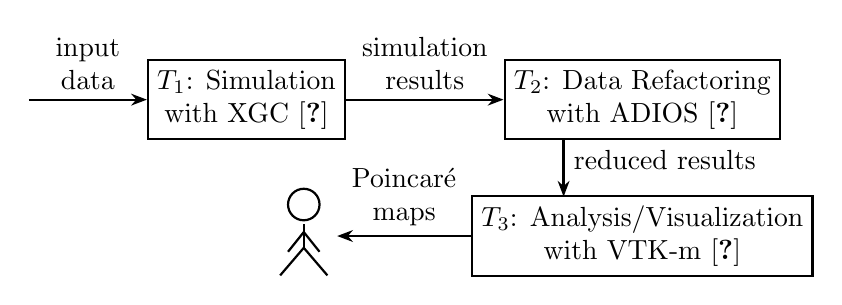
\begin{tikzpicture}[
    node distance=2cm,
    box/.style={rectangle, draw, thick, minimum width=2cm, minimum height=1cm, align=center},
    arrow/.style={-{Stealth[length=2mm]}, thick}
]

% Nodes
	\node[box, align=center] (task1) {$T_1$: Simulation\\with XGC~\cite{10.1063/1.5020792}};
	\node[box, right=of task1, align=center] (task2) {$T_2$: Data Refactoring\\with ADIOS~\cite{GODOY2020100561}};
	\node[box, below=0.7cm of task2, align=center] (task3) {$T_3$: Analysis/Visualization\\with VTK-m~\cite{7466740}};

% Stick figure user
\node[left=2cm of task3, xshift=0.3cm] (user-anchor) {};
\node[left=2cm of task3, yshift=0.4cm] (user) {};
\draw[thick] (user) circle (0.20cm); % head
\draw[thick] (user) ++(0,-0.25) -- ++(0,-0.30); % body
\draw[thick] (user) ++(0,-0.55) -- ++(-0.3,-0.35); % left leg
\draw[thick] (user) ++(0,-0.55) -- ++(0.3,-0.35); % right leg
\draw[thick] (user) ++(0,-0.35) -- ++(-0.2,-0.25); % left arm
\draw[thick] (user) ++(0,-0.35) -- ++(0.2,-0.25); % right arm

% Incoming arrow to Task1
\coordinate[left=1.5cm of task1] (input);
\draw[arrow] (input) -- node[above, align=center] {input\\data} (task1);

% Arrows with labels
\draw[arrow] (task1) -- node[above, align=center] {simulation\\results} (task2);
\draw[arrow] ($(task2)+(-1cm,-0.5cm)$) -- node[right, align=center, yshift=+0.1cm] {reduced results} ($(task3)+(-1cm,+0.5cm)$);
\draw[arrow] (task3) -- node[above, align=center] {Poincar\'e\\maps} (user-anchor);

\end{tikzpicture}

}
\end{center}
\caption{Example three-task chain for a fusion energy science application~\cite{9912722}.}
\label{fig:use_case}
\end{figure}

For fault-tolerance purposes, the authors in~\cite{10678736} propose using
approximate computing techniques to trade off output quality for
shorter execution times. While many such techniques are
available~\cite{10.1145/3716845, 10.1145/3711683}, they focus on data size
reduction using generic compression methods or methods specifically
designed for scientific datasets~\cite{10.1145/3733104}.  Regardless, some
or all of the tasks in the application come with different execution modes
that correspond to, e.g., different compression factors, different data
refactoring options, and different precision levels.  The above use case
provides the motivation for the formulation of the scheduling problem in
the next chapter.






% =========================================================
% 
% See highlights and speech bubbles in the PDFs
% 
% - Error-Controlled Lossy Compression...: BigData18-SZ2.0.pdf
% 	- A paper on lossy stuff for science (cited by paper below)
% 	- May have some data to get some actual values...
% 
% - RAPIDS: ...  (3588195.3592983.pdf):
% 	TLDR:A good ref and source of refs about approximate computing in science.
%              It's basically trying to pick good option for data resilience
% 
% 	- Paragraph/refs about why lossless is not sufficiently scalable
% 	- Paragraph/ref about lossy stiuff and why its good for science
% 	- Paragraph/ref about data refactoring: which is what they use
% 	- Fault-tolerance:
% 		- how to pick data encoding (erasure + multi-level
% 		  refactoring) to maximize fidelity and minimize overhead
% 		  given the probability of losing a storage system
% 
% - Hybrid Analysis...: Hybrid_Analysis.pdf
% 	- Not sure it's relevant at all
% 
% - Towards Resilience Near Real-Time...: Suter_Towards.pdf
%   - THE reference for "timely workflow execution". Two technniques:
% 	- Replicas: nice but costly - Data reduction: faster i/O, faster
% 	  computation 
%         - PROBLEM: Mention a deadline in seconds! And there are faults?  
%         - Mentions that algorithms could also be tweaked but say
% 	  it's better to do data-reduction 
%         - techniques:
% 		- lossy or lossless compression - data reduction (see papers above) 
%                 - perhaps decompress/reconstruct 
% 	- Their problem:
% 		- Deadline 
%                 - Maximum number of failures  (They do R replicas to tolerate R failures) 
%                 - Maximum resource budget
% 	- We can say we consider a more general problem?
% 


\section{Problem Statement}
\label{sec:problem}

\subsection{Application Model}
\label{sec:problem-application}

The application is a chain of $M{\geq}1$
tasks. Each task $T_i$, $i{=}1, \ldots, M$, takes input data,
performs a computation, and generates output data, as a three-step
sequence. Each successful execution of $T_i$ produces output data,
any of which may be used as input by an execution of $T_{i+1}$. 
Data is always written to and read from stable
storage.  An ``in-situ" execution in which the output data from a parent
task remains in RAM and can be accessed by the child task without
any I/O would simply amount to merging these two
tasks into a single task.


Error in application data is tolerated:  $T_i$ offers $K_i{\geq}1$
execution modes for different trade-offs between
execution time and output error. 
$T_i$ takes $x{\in}\N$ bytes of input with an error level $y{\in}[1,
+\infty)$, where 1 denotes no error.  We define execution mode $j$ for
$T_i$, $j{=}1,\ldots, K_i$, by three functions:
\begin{itemize}
\item $t^i_j(x,y)$: The compute time (not including I/O); 
\item $d^i_j(x,y)$: The size in bytes of the output data; and 
\item $e^i_j(x,y)$: The error level in the output data.  
\end{itemize}
\noindent
In practice, these functions may be independent of some of
their inputs (see the example in Table~\ref{tab:compression_example}).

\begin{table}[hb!]
    \caption{Example execution modes for a data compression task. $x$ is the input data size in bytes
	 and $y$ is the input data error.}
    \label{tab:compression_example}
    \begin{center}
    \begin{tabular}{|l|l|l|l|}
    \hline
    Execution mode & $t(x, y)$ & $d(x,y)$ & $e(x,y)$\\
    \hline
    no compression & $0$ & $x$ & $y$\\
    slow lossless compression & $2{+}10 x$ & $x/10$ & $y$\\
    fast lossless compression & $1{+}5 x$  & $x/2$  & $y$\\
    fast lossy compression    & $1{+}2 x$  & $x/20$ & $3y/2$\\
    \hline
    \end{tabular}
    \end{center}
\end{table}

Error propagates through inter-task data dependencies and
accumulates end-to-end.  Many previous works on the scheduling of
real-time, approximate computing applications employ the ``monotone" model
by which a task can reduce the error in its input data by performing
additional computation~\cite{259428}.  The above model can account for this
error reduction behavior by defining the $t$ and $e$ functions
appropriately.  For the use cases that motivate this work, as that in
Section~\ref{sec:use-case}, there is no possibility of error reduction
(i.e., $e^i_j(x,y){\geq}y$).

The execution of the application must complete by a deadline, $D{>}0$. The
\emph{output error} is defined as the minimum error across the output data
of all successful executions of $T_{M}$ (the last task).  If no 
execution of $T_{M}$ has succeeded by the deadline, then the 
output error is set to $\efail$, a user-defined value that quantifies
the penalty for returning no usable output by the deadline. The value of
$\efail$ is set to be larger than any achievable output error by a successful
execution of $T_M$. 

\subsection{Platform and Fault Model}
\label{sec:problem-execution}

The platform comprises $N$ homogeneous
processing elements (PEs), that each can execute only one task at a time.
A PE could be a single core that executes a sequential program,
a multi-core host that executes a multi-threaded program, or a set of compute
nodes that execute a parallel program.
Each PE reads/writes task data on a parallel file system,
with read bandwidth $B_r$ and write bandwidth $B_w$. In
practice, PEs can experience contention when accessing the parallel
file system concurrently. While contention is part of our simulation
model (for experiments), our analytical model assumes no
contention so that analytical developments remain tractable.

Task executions on PEs experience fail-stop failures (failed task executions do not produce usable
output data).  Each PE is subject to independent failures with 
exponentially distributed inter-arrival times with 
rate $\lambda$ ($\lambda{=}0$ corresponds to a failure-free system).  
Exponentially distributed failures are commonplace in the fault-tolerance
literature due to their memoryless property. Although failures are not
necessarily memoryless in real-world settings, assuming exponentially
distributed failures remains sensible in practice~\cite{8049007}. We assume
a single rate $\lambda$ regardless of a task's execution mode.  Some works
consider different failure rates for different execution modes~\cite{10.1145/2442087.2442094,10.1007/s11227-021-03764-x,10.1109/TC.2003.1183950}.  Considering different failure
rates for different modes in this work would merely entail simple
modifications to the recursive formulas presented in
Section~\ref{sec:onehost:solution}.

Following a failure, the affected PE cannot resume computing for $R{\geq}
0$ seconds. This \emph{restart overhead} corresponds to acquiring a spare
host (due to a hardware failure), rebooting the host (due to an OS
crash), or simply restarting a task (due to a software bug).  As
commonly done in the literature, we assume a single restart overhead and do
not distinguish different types of failures. Here again, doing so would
entail straightforward (if tedious) modifications to the recursive
formulas presented in Section~\ref{sec:onehost:solution}.

A key technique to handle fail-stop failures is rollback/recovery, by
which a task is restarted if it fails~\cite{10.5555/2811302}.  A common
question is that of whether and when a task should
checkpoint its state to stable storage to avoid rolling back the entire
computation when a failure occurs~\cite{BAUTISTAGOMEZ2024315}.  In this
work checkpointing is built into the application because each task reads
its input and saves its output to stable storage.  Our model can easily
be extended to consider a task that implements its own checkpointing:
replace the task by a chain of tasks, each of which corresponds to the
execution between two checkpoints. All tasks in this chain, except the
first, would read their input from stable storage only when restarted
after a failure, which would require minor changes to the recursive
formulas presented in Section~\ref{sec:onehost:solution}.  Besides
rollback/recovery, another key technique is replication, by which backup
tasks are executed on different PEs to increase the chances that at least
one replica will succeed~\cite{10.5555/2811302}.  In this work, we 
use both rollback/recovery and replication.

%There are works that say "checkpoint more the closer to the deadline": we
%don't do that. cite? (ref [68] in 3589950.pdf) Discuss in related work?
%Future work? Ignore?


\subsection{Scheduling Problem}
\label{sec:problem-scheduling}

We consider the problem of \emph{minimizing the expected output error} for
a single invocation of the application, released at time zero and subject
to an end-to-end deadline $D$.  As seen in our motivating use case in
Section~\ref{sec:use-case}, the application is intended to be invoked
periodically. But successive invocations do not overlap, no unfinished work
carries over beyond a deadline, and all PEs are available at the beginning
of each invocation.  Each invocation can thus be scheduled independently
using the same strategy. In other words, only the deployment of the
application is periodic, not its scheduling.

The scheduling problem is offline because application and platform specifications 
are known in advance.  But because
failures are stochastic, a scheduling strategy should be
adaptive and make decisions that account for execution events at runtime.
Therefore, we consider scheduling strategies that are invoked at time zero
and also in response to task completions, task failures, and PEs becoming
available.  Scheduling decisions can consist of aborting current task executions
(making PEs immediately available) or selecting which tasks to execute with
which execution modes.  We define an \emph{optimal strategy} as one in
which each decision minimizes the expected output error given the current
state of the application execution and the time remaining until the
deadline. The scheduling problem then is to determine an optimal
strategy.



\begin{proposition}
\label{prop:np}
The above scheduling problem is NP-hard, even for a one-PE, failure-free platform
with zero I/O costs, two modes per task, and
zero restart overhead.
\end{proposition}

\begin{proof}
With no failures, the execution is non-stochastic. All scheduling decisions
can be made at time zero and, with one PE, we can restrict ourselves to
strategies that execute each task exactly once with one mode.  Let us
prove the NP-completeness of the decision problem: does there exist a
strategy that can achieve an output error of at most some threshold $\tau$?
The problem is in NP because, given the list of the chosen execution modes,
one can compute the overall execution time and output error in polynomial
time.  We prove NP-completeness via a reduction from 0-1
\knapsack~\cite{GareyJ79}.

Consider an instance of 0-1 \knapsack with $m$ items, where item
$i{=}1,\ldots,m$ has weight $w_i$ and value $v_i$. The knapsack capacity is
$W$, and for $V{>}0$ we consider the problem of deciding whether a solution
exists with total value ${\geq}V$.  We construct an instance
of our scheduling decision problem as follows. We consider an $m$-task
chain in which task $T_i$, $i{=}1,\ldots,m$ has two execution modes:
(i)~\emph{fast}: execution time $t(x,y){=}1$, output size $d(x,y){=}0$, 
and error $e(x,y){=}y{+}v_i$ (i.e., introduced additive error); and (ii)~\emph{slow}: execution
	time $t(x,y){=}1{+}w_i$, output size $d(x,y){=}0$, and error
function $e(x,y){=}y$ (i.e., no introduced error).
We set the deadline to $D{=}m{+}W$, the size of the initial input to 0,
and the error of the initial input to 1. 
Let us define $\tau{=}1{+}V_{\Sigma}{-}V$, where
$V_{\Sigma}{=}\sum_{i=1}^m v_i$.  We consider the problem of deciding whether
there exists a strategy for which the chain's output error is
${\leq}\tau$.  We define $e_f{=}2{+}V_{\Sigma}$, so that a chain execution
that does not complete by the deadline leads to error strictly greater than
$\tau$.  This construction is computable in polynomial time.

Let $S$ be the set of tasks that are executed with their slow execution
mode, as decided by the strategy. 
The application execution finishes by deadline $D$ when:
$$
\sum_{i \notin S} 1 + \sum_{i \in S} (1 + w_i) \leq m + W\;,
\text{i.e., when}
\;\sum_{i \in S} w_i \leq W .
$$
The chain's output error is:
$$
1 + \sum_{i \notin S} v_i = 1 + V_{\Sigma} - \sum_{i \in S} v_i = \tau + V - \sum_{i \in S} v_i \;.
$$
Therefore, the chain's output error is ${\leq}\tau$ if and only if $\sum_{i
\in S} v_i{\geq}V$.  In other words, the answer to the scheduling decision
problem is yes if and only if the answer to the knapsack decision problem is yes,
completing the reduction.
\end{proof}





\chapter{Experimental Methodology}
\label{sec:methodology}

Our simulator, application workloads, simulation results, and results processing scripts are publicly available~\cite{HIDDEN_URL}.

%are publicly available~\footnote{URL omitted for double-blind review.}.



\section{Application Workloads}

Some of our results are illustrated for the fusion
science application in Fig.~\ref{fig:use_case}. Tasks
$T_1$, $T_2$, and $T_3$ have four, four, and three execution modes, respectively,
each described by affine $t$, $d$, and $e$ functions.  These particular
execution modes and affine functions are based on results in~\cite{9912722}
and on information provided to us by the authors.  
%Although we have
%used some best guesses for some coefficients in these functions, we
%believe our specification to be representative of a practical use case.

We also evaluate heuristics over a large set of synthetic application
configurations.  A synthetic configuration is generated as follows. We
randomly sample the number of tasks $M{\in}\{2,3,4,5\}$. For each task
$T_i$ we randomly sample its number of modes $K_i{\in}\{2, 3, 4\}$. We then
generate a first ``safe" ($s$) execution mode (fast, high error)
and a last ``risky" ($r$) execution mode (slow, low error) as
follows, omitting arguments on which a function does not depend:

\begin{minipage}{0.39\columnwidth}
\begin{itemize}[leftmargin=0pt, labelindent=0pt, labelsep=0.3em]
\item $t^i_s{=}u_{50, 600}$
\item $d^i_s{=}\lceil u_{10^{10}, 10^{12}} \rceil$
\item $e^i_s(y){=}u_{3, 10} \cdot y$
\end{itemize}
\end{minipage}
\begin{minipage}{0.55\columnwidth}
\begin{itemize}[leftmargin=0pt, labelindent=0pt, labelsep=0.3em]
	\item $t^i_r{=}u_{2 \cdot t^i_s , 6 \cdot t^i_s}$
	\item $d^i_r{=}\lceil u_{0.01 \cdot d^i_s, 0.3 \cdot d^i_s} \rceil$
	\item $e^i_r(y){=}u_{1, \min(0.6 \cdot e^i_s(1), e^i_s(1) - 0.5)} \cdot y$
\end{itemize}
\end{minipage}~\\

\noindent
where $u_{a,b}$ denotes a value sampled once from the uniform distribution 
on $[a,b] \subset \mathbb{R}$.  Additional modes are generated between the safe and risky
modes using linear equidistant interpolation. In practice, the $t$ and $d$
functions are likely non-constant (as in our fusion science use
case). However, using constant functions, especially in the input size,
makes it straightforward to generate a broad range of configurations
in which no execution mode is trivially dominated by another.

The intervals for the uniform distribution are selected empirically
to ensure that the application configurations are diverse enough that
different scheduling algorithms can make a wide range of reasonable
decisions.  For each generated application configuration we
compute $p_s$, resp. $p_r$, the probability that the execution on a single
PE succeeds by the deadline when using only safe, resp. risky, execution
modes.  $p_s$ and $p_r$ are computed using dynamic programming (see
Chapter~\ref{sec:onehost}) using the same $D$, $\lambda$, $R$, $B_r$, and
$B_w$ values as that used in simulation.  To eliminate trivially easy or
hard cases, we filter out configurations with $p_s{<}0.15$, $p_s{>}0.85$,
or $p_r{<}0.01$.  The $D$ and $\lambda$ values merely establish a common
time scale; failure behavior is driven by the overall application
execution time relative to the deadline, $D$, and to the mean time between failures,
$1/\lambda$.  Our synthetic configurations do not aim to model any
specific workload. Instead, they define a set of scenarios with different
relative execution-time, data-size, and error magnitudes,  over which
different scheduling principles can be compared systematically.

%\TODO{Perhaps (likely cannot due to space) add data to justify that the configurations are really diverse....}

\section{Simulation Methodology}

Our simulator builds on a simulation framework designed to model real-world
software/hardware platforms, and in particular network and I/O operations,
accurately.  Scheduling works in the literature, like this one, typically
use an abstract model of I/O operations, where transfer time is simulated as
the data volume divided by some nominal bottleneck bandwidth, to render
analytical developments and algorithm design
tractable~\cite{10.1145/2501654.2501664, 7965082}. Our simulator supports
two I/O simulation modes.  Its ``model-consistent" mode enforces the above
abstract model, and is used to validate our implementation. Its
``realistic" mode uses realistic simulation models that account for
protocol and contention effects.  Unless specified otherwise, simulation
results are obtained with the realistic mode.  Each invocation of the
simulator takes in a full specification of the scheduling problem, as well
as a seed value for the random number generator used to inject failures
into the execution.  For a given instance of the scheduling problem,
simulation results are obtained for different seeds, i.e., different
failure traces.

Unless specified otherwise, analytical/simulation results are 
for $D{=}10^4$, $\lambda{=}10^{-3}$, $R{=}0$, $B_r{=}$2 GB/s, and $B_w{=}$1 GB/s.



\section{One-PE Platform}
\label{sec:onehost}

With a single PE, only one task can execute at a time and rollback/recovery is the only way to cope with failures.  For a single task, with fixed execution time and zero restart overhead, computing the probability of completion by a deadline is non-trivial as it requires characterizing the ``longest gap" distribution of a Poisson process~\cite{OMWONYLEE2020124194}.  Furthermore, when considering a chain of tasks there is a continuum of possible values for the time remaining until the deadline at the next scheduling decision.  To make the continuous-time scheduling problem tractable, we thus discretize time. 
For a given application, we use dynamic programming to precompute scheduling decisions in time polynomial in the number of discrete time intervals, and $O(1)$-time scheduling decisions at runtime.


\subsection{Scheduling Strategy}
\label{sec:onehost:solution}

Let time be discretized as a sequence of time steps 
of duration \deltat, so that all time durations are
integral numbers of time steps. The execution time for 
execution mode $j$ of task $T_i$, for $x$ bytes of input data 
with error level $y$ is then: 
$$
m^i_j = \left\lceil \frac{x/B_r + t^i_j(x,y) + d^i_j(x,y)/B_w}{\deltat} \right\rceil ,
%m^i_j = \left\lceil (x/B_r + t^i_j(x,y) + d^i_j(x,y)/B_w) / \deltat \right\rceil ,
$$
\noindent
where the numerator is the time to read the input, to perform
the computation, and to write the output. 

Let us consider an execution that conforms to a ``first-output" policy
by which a task is never re-executed once it has completed
successfully once.  This implies that the application execution stops as
soon as one execution of task $T_M$ has succeeded. Imposing this
restriction makes the recursion hereafter more tractable and, more
importantly, limits the state space size of the corresponding dynamic program.

We define $E(i, x, y, n)$ as the optimal expected error (with discretized time)
when executing $T_{i}$ to
$T_{M}$ for $i{=}1,\ldots,M$, where the input to $T_{i}$ is $x$ bytes
with error level $y$, given that there are $n$ time steps until the
deadline.  If $\forall j\; m_j^i{>}n$, then $E(i, x, y, n){=}\efail$, since
there is no possibility of completing $T_{i}$ by the deadline.
Otherwise, recursively:
\begin{multline}
\label{eq:dp1}
E(i, x, y, n) = 
    \min_{1\leq j \leq K_i,\; s.t.\; m_j^i \leq n} \big[\\
\psuc{m_{j}^i} \times E(i+1, d_j^i(x,y), e_j^i(x,y), n - m_j^i) + \\
	\sum_{u=0}^{m_j^i - 1} p_u E(i, x, y, \max(0, n - u - 1 - \lceil R/\deltat \rceil)) \big],
\end{multline}
\noindent
where $p_u{=}\psuc{u}{-}\psuc{(u+1)}$, i.e., the probability that a failure
occurs during time step $u$, where time step 0 is the first time step. 
The above expression is the minimum expected error over all feasible execution modes used for the upcoming execution of $T_{i}$.  The first term 
is for the case in which there is no failure during the execution of $T_{i}$ with execution mode $j$, which happens with probability
$\psuc{m_{j}^i}$. In this case, the execution will proceed with
$T_{i+1}$, with input data size and error level based on the
output from $T_{i}$, and with 
$m_j^i$ fewer time steps remaining until the deadline. The second term considers all time steps at which the
execution of $T_{i}$ can fail. Failing during time step $u$ happens with
probability $p_u$ and will cause a re-execution of $T_i$ but with
$u{+}1{+}\lceil R/\deltat \rceil$ fewer
time steps until the deadline.  The base case is
simply $E(M+1, x, y, n) = y\;$.

%$E(M, x, y, n)$, is when only $T_{M}$ is left to execute. 
%$E(M, x, y, n)$ is equal to $\efail$ if $\forall j\; m_j^M{>}n$  (i.e., there are no feasible execution modes). Otherwise, recursively:
%\begin{multline}
%E(M, x, y, n) = \min_{1\leq j \leq K_M,\; s.t.\; m_j^M \leq n} \big[\psuc{m_{j}^M} \times e_j^M(x,y)\\
%	+ \sum_{u=0}^{m_j^M - 1} p_u E(M, x, y, \max(0, n - u - 1 - \lceil R/\deltat \rceil)) \big].
%\end{multline}
%The only difference with Equation~\eqref{eq:dp1} is that if $T_M$ succeeds
%with execution mode $j$, then the recursion ends and the output error
%s simply $e_j^M(x,y)$.

The above recursion provides a dynamic programming solution for
precomputing all scheduling decisions.  The initial decision is to select
an execution mode that attains the minimum in the expression for $E(1,x_0, y_0,
H)$, where $x_0$ and $y_0$ are the size and error of the input to task
$T_1$, and $H{=}\lfloor D/\deltat \rfloor$.  Note that the number of time
steps until the deadline is rounded downward, while we round task execution
times and restart overheads upward, so that an execution computed in
discretized time is guaranteed to be feasible in continuous time.  Using
memoization, all reachable values $E(i, x, y, n)$, together with the
execution modes attaining their minima, can be precomputed and stored in a
table.  At runtime, whenever the PE is idle, the execution mode for the
current state $(i, x, y, n)$ can be selected in $O(1)$ time by looking up
the table.

Let us denote by $Q$ the number of possible size/error pairs for the input
provided to all tasks, and let $K{=}\max_i K_i$. The time complexity for
the above algorithm is $O(KQH^2)$, and the size of the computed table is
$O(QH)$. The table could be compressed by storing, for each state $(i,x,y)$,
maximal intervals of values for which
the selected mode is unchanged.  Regardless, for a fixed application
specification, the time and space complexities are pseudo-polynomial in
the numerical deadline.  Although $Q$ may be exponential in the number of
tasks, the algorithm remains practical (see results in the next section).
Besides, for a given application and failure rate, the algorithm is
invoked offline only once, and the computed table can be reused for all
executions of the application.



%\HC{This following paragraph could be removed or heavily modified based on the TODOs hereafter}
%When the application consists of a single task, one can prove that the set
%of time steps until the deadline can be partitioned into time intervals,
%and that one can compute in pseudo-polynomial time the optimal execution
%mode to use when a decision is made at any point in each of these
%intervals.  In this manner, one can precompute a table of size $O(K_1)$,
%and at runtime one can select the optimal execution mode to use for the
%next task execution with complexity $O(\log K_1)$ using binary search.
%This result, however, does not seem to generalize to chains of more than
%one task. We thus omit it here due to lack of space.

Recall that the above approach is for a first-output policy. Due to the randomness of
failures the application may complete well ahead of the deadline.  A
natural idea is then to use opportunistic \emph{temporal redundancy} and
attempt subsequent application executions. Integration of this idea in our
recursion would require an enlarged state space.  Instead, we perform
temporal redundancy as a separate re-execution step after $T_M$ completes.
Each such re-execution is computed while excluding task mode sequences
that cannot possibly improve on the error level achieved by the previously
completed execution. It is straightforward to remove these execution modes
from consideration and, provided any viable execution modes remain, apply
our scheduling strategy again. The extent to which this temporal redundancy
technique is useful depends on the application specification, the failure
rate, the restart overhead, and the deadline. In our experimental results,
when using this technique, we always restart the application
from task $T_1$.  Assuming that
intermediate task output data from the previous execution are still
available in stable storage, the re-attempted execution could start
with task $T_{i_0}$, $i_0 > 1$. We leave investigating this possibility, including
the problem of determining the best $i_0$, for future work.


\subsection{Discretization Selection}

A practical question is: what value of $\deltat$ should be used?  A
smaller $\deltat$ value yields a better approximation of the continuous-time problem,
but leads to higher complexity due to a larger number of time steps.  
Although the algorithm needs to be invoked only once, a user could still wish
to determine the largest value of $\deltat$ that leads to accuracy within
some tolerance.

The developments in the previous section actually compute a pessimistic
upper bound on the optimal continuous-time expected error for the first-output
policy.  This is because the dynamic program is invoked for the deadline
rounded downward, all task durations $m^i_j$ are rounded upward, the
restart overhead is rounded upward, and a failure at any point in a time
interval ``wastes" that entire interval.  Small modifications make it
possible to compute an optimistic lower bound: invoke the
dynamic program for the deadline rounded upward; round all $m^i_j$ task
durations downward; and replace $n{-}u{-}1{-}\lceil R/\deltat\rceil$ by
$n{-}u{-}\lfloor R/\deltat \rfloor$ in the recursive expressions.  Note
that for $u=0$, if $\lfloor R / \deltat \rfloor = 0$ there is a self-loop in
the recursion. In this case we disregard the $u=0$ term in the summation
(and renormalize probabilities).

\begin{figure}[ht!]
	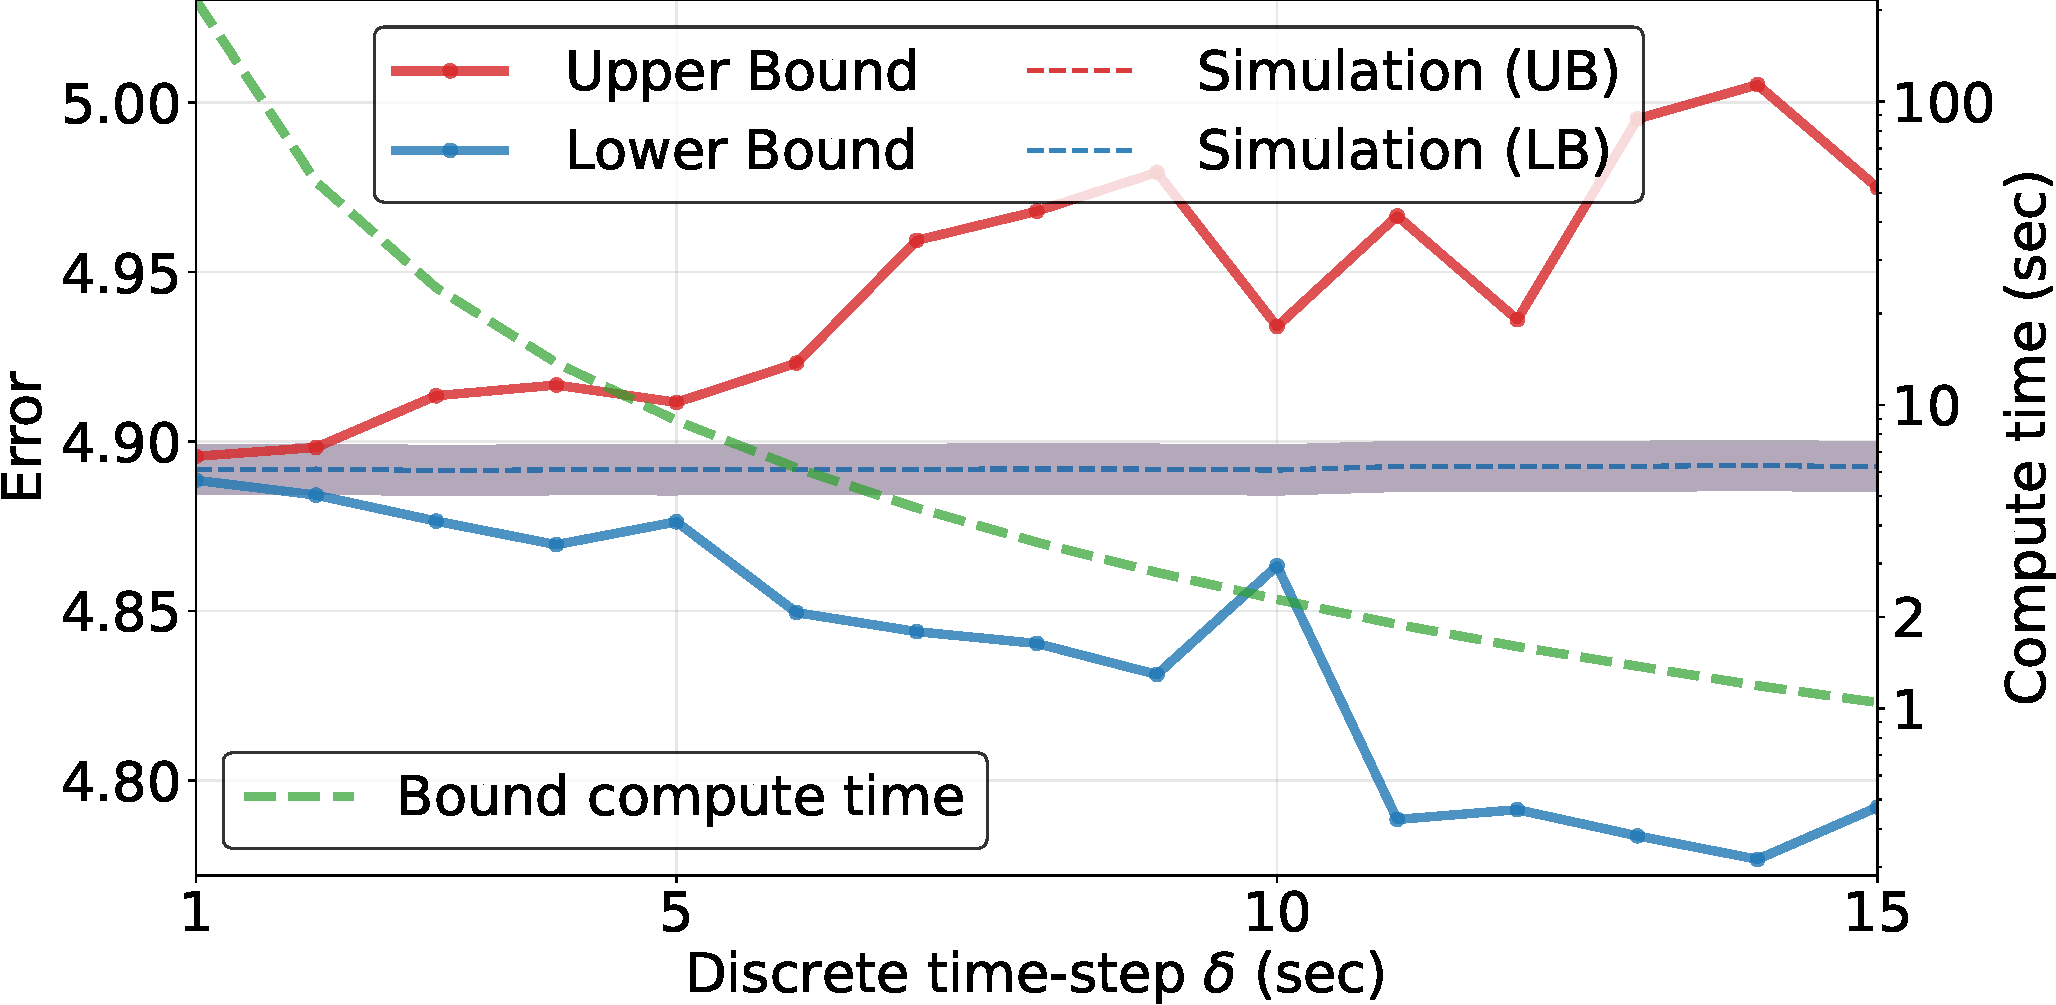
\includegraphics[width=\columnwidth]{./figures/delta_t_results.pdf}	
	\caption{Expected error bounds, sample simulated
	error for 5 million repeats (95\% confidence interval shown by
	shaded region), and bound computation time vs. $\deltat$, for the
	fusion science use case in Section~\ref{sec:use-case}.}
	\label{fig:delta_t}

\end{figure}

In practice, a user would pick a value for \deltat so that the difference
between the two bounds is below some threshold, and then make scheduling
decisions according to the dynamic program for the lower bound or for the
upper bound. For instance, Fig.~\ref{fig:delta_t} plots the two bounds
vs. \deltat for the use case in Section~\ref{sec:use-case}.  As expected,
the distance between the two bounds increases as \deltat increases. But
the increase is not monotonic, as seen in the jagged shape of the
curves. This behavior is easily explained by discretization effects. 
For instance, in the dynamic
program for the upper bound, a task of duration $t$ is considered to take
time $\lceil t{/}\deltat\rceil{\times}\deltat$, which happens to be a
non-monotonic function of \deltat. The plot also shows the time to compute
the table (on a single 2.10 GHz core), using our implementation of the recursion in
the previous section. The execution time decreases sharply as \deltat
increases (the rightmost vertical axis is on a logarithmic scale).  It is thus
feasible to compute tight bounds relatively quickly. For instance, for
$\deltat{=}5$, the computation time is $\sim$8.9s, and the distance
between the two bounds is $\sim$0.72\% of the upper bound. 

We also wish to verify that our analytical bounds are consistent with our
simulator's implementation. To this end, Fig.~\ref{fig:delta_t} also shows
the simulated sample mean error and its 95\% confidence interval, over 5
million trials, each for a different random seed (the simulator is executed in
``model-consistent'' mode, as described in Section~\ref{sec:methodology}).
The simulated scheduling algorithm uses results produced by the dynamic
program for the lower or for the upper bound (both results are shown but
coincide almost exactly) to make scheduling decisions, without using
temporal redundancy.  Results in the figure confirm that the simulated
sample mean error lies between the two bounds, and so does the confidence
interval provided \deltat is large enough.

All results in the rest of this paper are obtained with $\deltat{=}5$. The
above results show this value to be sufficient to achieve high accuracy for
our deadline $D{=}10^4$ (i.e., 2,000 discretized time steps). Recall
that this is the deadline used in all our experiments, unless specified otherwise.


\subsection{Platform Provisioning for Parallel Tasks}
\label{sec:data_parallel}

In practice, application tasks may be
parallel programs that can be executed on $n$ homogeneous compute nodes
(e.g., an allocation/partition in a commodity cluster).  In this section we
consider $n$ gang-scheduled compute nodes as a single PE that executes
tasks one at a time and fails with rate $n{\times}\lambda_{node}$, where
$\lambda_{node}$ is the failure rate of a single node. (In
Section~\ref{sec:multihost}, we consider the case of $N$ independently
schedulable PEs.)

\begin{figure}[ht!]
	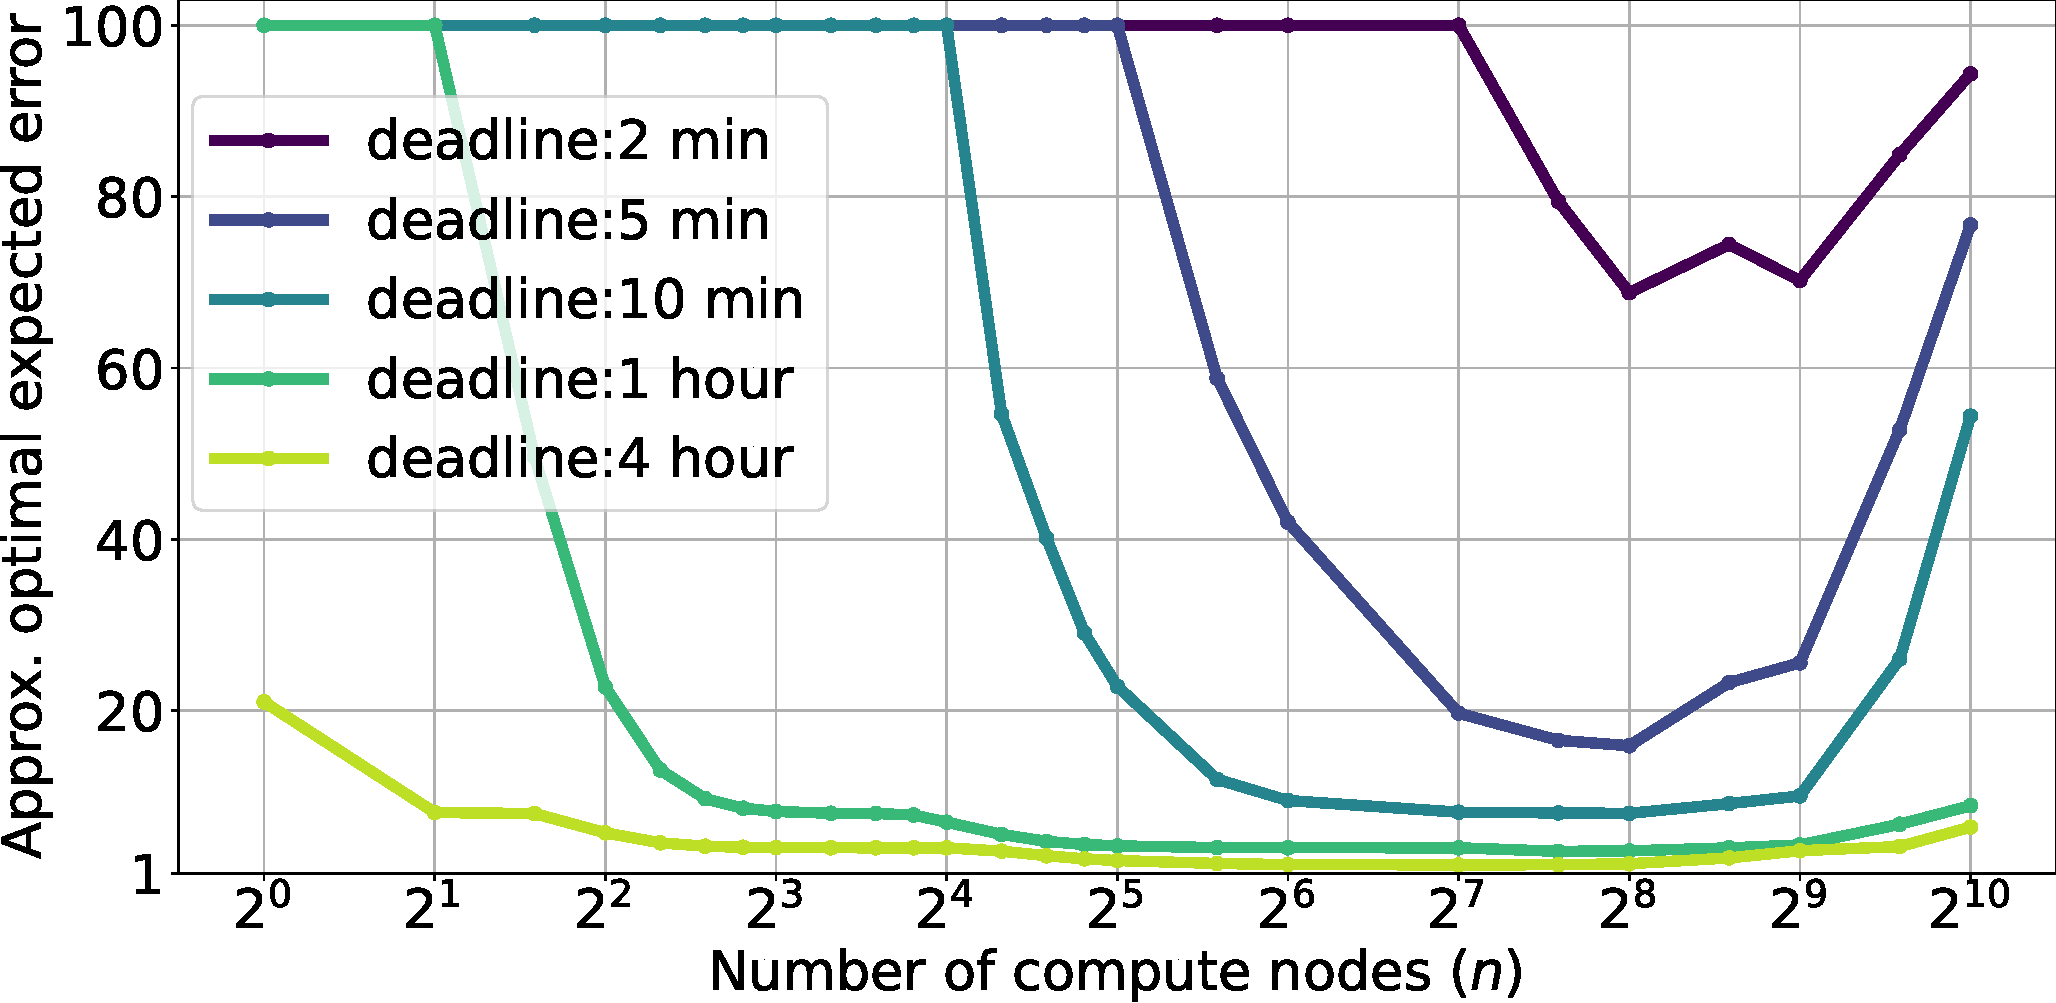
\includegraphics[width=\columnwidth]{./figures/data_parallel_results.pdf}	
	\caption{Approximate optimal expected error vs. number of compute nodes for different deadlines, for the fusion use case in Section~\ref{sec:use-case}.}
	\label{fig:data_parallel}
\end{figure}

Fig.~\ref{fig:data_parallel} shows the approximate optimal expected
error, as computed using the results in Section~\ref{sec:onehost:solution},
vs. $n$ for our fusion science use case.  Using a simple Amdahl parallel
speedup model, the fraction of the sequential execution that is
parallelizable is $0.89$, $0.99$, and $0.99$ for tasks $T_1$, $T_2$, and
$T_3$, respectively. These values are based on results
in~\cite{9912722} and on information provided to us by the authors.  As
seen in the figure, the tighter the deadline, the more compute nodes are
necessary to achieve an expected error below \efail (which is set to 100
in these experiments). For instance, doing so
for a 5-minute deadline requires $n{>}32$ compute nodes.  
But using as many compute nodes as possible is not advisable because the
failure rate increases with $n$.  There is thus a ``sweet spot" where
$n$ is large enough for parallelization to be useful but small enough that
failures are not too frequent.  Note that, for the shorter deadlines, the
curves appear more jagged. This is because
$\deltat{=}5$ is larger relative to the deadline, leading to a coarser 
discretization (using a smaller $\deltat$ value
would yield more precise approximations
of the optimal expected error for these shorter
deadlines). Overall, such results 
allow a user to make informed decisions, e.g., select a value of $n$ and a
deadline that achieve a desirable compromise between hardware cost,
timeliness, and expected error.

%\subsection{In-Situ Executions}
%
%Another application of our results is provide a sound comparison of different execution
%options. For instance, one may wish to determine whether on should execute
%that task chain in an ``in-situ" manner, i.e., keeping all task input/output data
%in memory. While this reduces application execution time by removing all I/O
%operations, but requires a re-execution from scratch when a failure occurs.
%
%\TODO{This section is perhaps unnecessary. We should update the code to allow in-situ executions. Done with the USE CASE}


\subsection{Evaluation of Simple Heuristics}
\label{sec:onehost:heuristics}

Our dynamic programming approach is usable in practice. It also
provides a reference against which heuristics can be compared and evaluated.
This is useful to determine which scheduling principles are effective in the 
one-PE case, and may be worth reusing in the multi-PE case.

We consider four criteria for selecting a task's execution mode:
(\errorlevel)~the lowest error level;
(\probsuccess)~the highest probability of success by the deadline; (\ratio)~the
highest ratio of probability of success to error level; and (\expectederror)~the
lowest expected error by the deadline. Criterion \expectederror criterion is computed using the recursion in Section~\ref{sec:onehost:solution}, while criteria \probsuccess and \ratio
are computed using modified versions of that recursion.  We then consider two categories of heuristics:
\begin{compactitem}	
	\item \textbf{Nearsighted} (\textsc{Ns}) - When selecting the execution mode for the next task using the chosen criterion, assume that this task is the last task in the chain. 
	\item \textbf{Foresighted} (\textsc{Fs}) - At the onset of the application execution, 
	analyze each possible combination of execution modes for all tasks and select 
	the combination that optimizes for the chosen criterion.
\end{compactitem}
\noindent
We denote each heuristic by its category and criterion, e.g., heuristic
\foresighted-\expectederror is the foresighted heuristic that uses the
lowest-expected-error criterion. All these heuristics are static, i.e.,
once an execution mode has been decided for a task, that same mode is used
for any re-executions of that task.  Finally, we consider a baseline
heuristic, \random, that picks task execution modes randomly,  for a total
of $4{\times}2{+}1{=}9$ heuristics.



We evaluate our dynamic programming approach, which we denote by \dynamic, along
with the above nine heuristics in simulation, for 500 different synthetic
application configurations and 20 random trials per configuration. We use
two different $\efail$ multipliers, i.e., $\efail$ is set to either 2$\times$ or
5$\times$ the highest possible error that a successful application execution can
achieve.  All findings and rankings hereafter are unchanged
when considering results for different multiplier values separately, and we
only discuss combined results.  The use of temporal redundancy can only be
beneficial, and our results show improvements in mean error ranging from 0\% to
8.97\% for all our heuristics, with an average improvement of 2.18\%. In
all that follows, we only discuss results with temporal redundancy enabled.

\begin{figure}[ht!]
	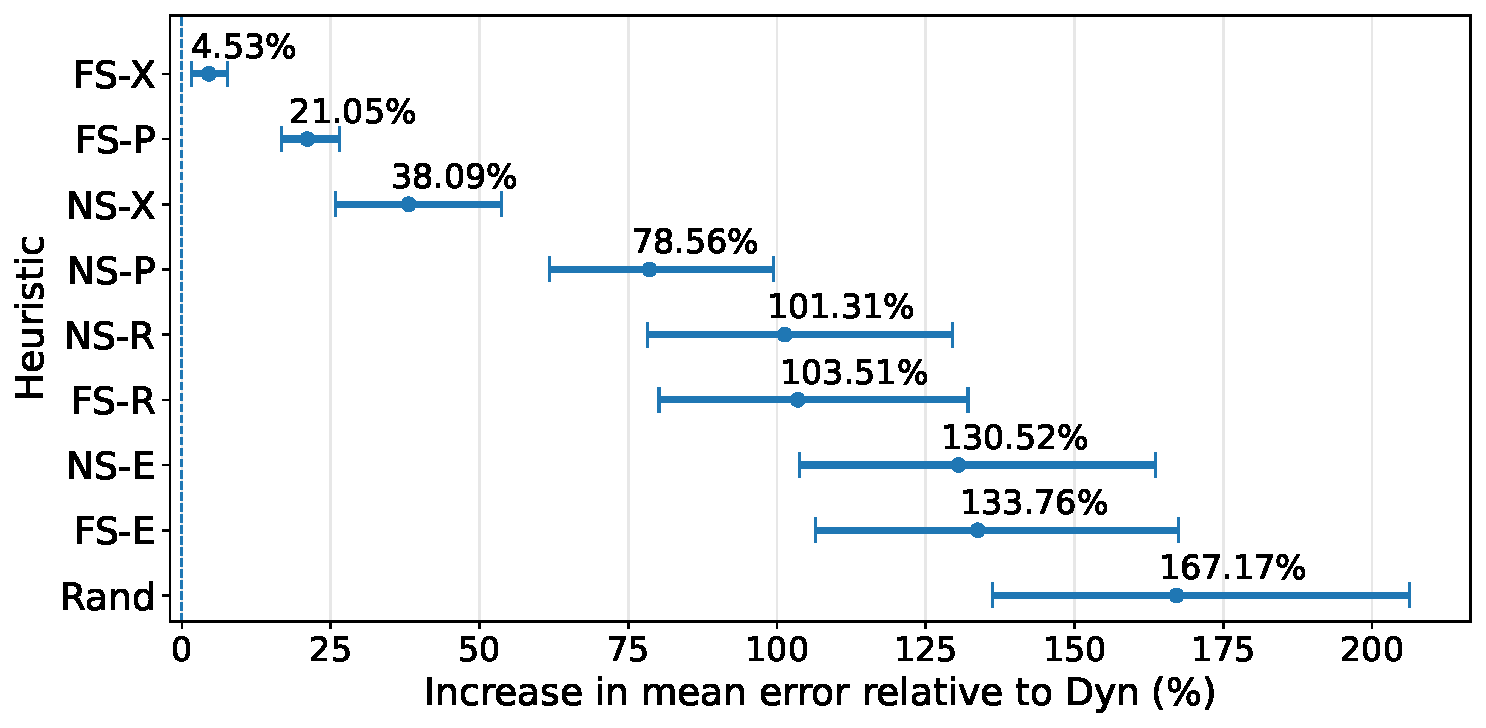
\includegraphics[width=\columnwidth]{./figures/relative_error_vs_dynamic.pdf}
	\caption{Mean error increases relative to the dynamic programming approach in the one-PE case (95\% paired-bootstrap confidence intervals shown).}
	\label{fig:one_host_results}
\end{figure}


We compare a heuristic $H$ to \dynamic using
the relative difference in expected error, $(\mu_H-\mu_{\dynamic})/\mu_\dynamic$,
where $\mu$ denotes the achieved expected error.  We
estimate this quantity using the corresponding sample means and compute a
95\% paired percentile-bootstrap confidence interval. 
Fig.~\ref{fig:one_host_results} shows these intervals
for all heuristics. \dynamic outperforms all heuristics, since no confidence interval contains the value zero. As expected, \random
performs the worst. We find that among the four criteria, the ranking from
best to worst is \expectederror (expected error), \probsuccess (probability of
success), \ratio (probability of success to error level ratio), and
\errorlevel (error level). This is also expected because criterion
\expectederror is the most directly related to the mean error objective, while
criterion \errorlevel, which comes last, is the least related. 
In terms of heuristic
categories, for the bottom two criteria (\ratio and \errorlevel), the
\nearsighted and \foresighted versions perform similarly, with a small
advantage to \nearsighted. However, for the top two criteria (\expectederror and \probsuccess), the
\foresighted heuristic outperforms the \nearsighted version.  This
intuitively makes sense: the quality of the criterion magnifies the
quality of longer-term planning.

Overall, the top-performing heuristic is \foresighted-\expectederror
(foresighted with the lowest expected error as the criterion), with a mean error increase
of 4.53\% relative to \dynamic. In our results, out of 20,000 experiments, 
\foresighted-\expectederror and \dynamic tie in 11,584 cases, \dynamic
wins in 7,106 cases and loses in 1,310 cases. 
\dynamic is not guaranteed
to produce the lowest error for every particular failure trace: it
minimizes expected error rather than the error for a particular realization
of the failure process. 
To ascertain the sensitivity of the above results to the
(number of) samples, we performed 500 random split-half analyses (keeping
all experiments associated with the same application configuration in the
same half). \dynamic ranked first and \foresighted-\expectederror ranked second
in 100\% of the half-samples.




\section{Multi-PE Platform}
\label{sec:multihost}


In this section we consider a platform with $N{>}1$ independently
schedulable PEs.  A direct extension of the dynamic programming approach in
the previous section would entail tracking the joint state of all task
executions on all PEs. The state space is thus combinatorial in $N$
(exponential with a straightforward representation), making the algorithm
no longer pseudo-polynomial time (if $N$ is considered part of the input).
Even for fixed $N{>}1$, its time and space requirements would likely be
prohibitive in practice.  Proposition~\ref{prop:np} establishes weak
NP-hardness for the one-PE case. Whether a stronger complexity result is
possible for the multi-PE case is an open question. Hereafter, we
present several heuristics, some of which build on the one-PE dynamic program.

\subsection{Heuristics}
\label{sec:multi-host:heuristics}

As in the one-PE case, we consider the
\dynamic heuristic (which is executed independently at each PE) and the
\random heuristic.  Section~\ref{sec:onehost:heuristics} describes eight
one-PE heuristics: nearsighted (\nearsighted) vs.  foresighted
(\foresighted), using one of four different criteria to select execution
modes (\errorlevel, \probsuccess, \ratio, \expectederror).  We extend these
heuristics to account for the simultaneous availability of all $N$ PEs at
time zero: given the $K{\geq}1$ possible execution modes for $T_1$, the
goal is to determine $n_1, n_2, \ldots, n_K$, where $n_j$ is the number of
PEs that will execute $T_1$ with mode $j$.  We initially set all $n_j$'s to
zero and compute their values greedily.  At each step, we
consider the option of incrementing one of the $n_j$'s (by one), leaving
all others at their current value.  Among these $K$ options, we pick the
one that leads to the best value of the scheduling criterion used by the
heuristic. This process is repeated until $\sum_{j=1}^{K} n_j = N$.
Hereafter we refer to these eight multi-PE heuristics as the ``greedy"
heuristics.

\subsection{Temporal Redundancy}

The design space for temporal redundancy is larger than in the one-PE case,
and we consider three options: 
\begin{compactitem}
	\item \textbf{Independent} (\independent) -- Use temporal redundancy 
	independently at each PE whenever it becomes idle due to 
	$T_M$ completing successfully.

	\item \textbf{Dependent} (\dependent) -- When $T_M$ completes successfully at a PE,
	  all PEs whose current executions cannot possibly achieve a lower error (due
	  to error levels achieved so far) abort their executions and apply
	  temporal redundancy.

	\item \textbf{Aggressive} (\aggressive) -- When $T_M$ completes successfully
	at a PE, all other PEs abort their
	executions and apply temporal redundancy.

\end{compactitem}


\subsection{Reactive Rescheduling}

With multiple PEs, there is an opportunity for
\emph{reactive rescheduling}: upon the completion 
of a task execution at a PE, other PEs can abort their ongoing task
executions and perform new scheduling decisions.  We consider three
options:

\begin{compactitem}
	\item \textbf{Off} (\off) -- No reactive rescheduling.

	\item \textbf{Variant} (\variant) -- Upon completion of task $T_i$ at
	PE $p$, if the ongoing application execution at PE $q{\neq}p$
	cannot achieve a lower overall error than the execution at PE
	$p$, then $q$ aborts its execution. An application execution
	is then restarted on PE $q$, but starting at task $T_{i+1}$. The
	input data provided to task $T_{i+1}$ is the output data from
	the execution of task $T_{i}$ at PE $p$.

	\item \textbf{Aggressive} (\aggressive) -- Upon completion of task $T_i$ at
	PE $p$, all other PEs abort their ongoing application executions
	and restart their executions at task $T_{i+1}$. The input data
	provided to task $T_{i+1}$ is the output data from the execution of
	task $T_{i}$ at PE $p$.
\end{compactitem}
\noindent

\subsection{Evaluation Methodology}

We define a scheduling strategy as a combination of \emph{design choices},
\strategy{A}{B}{C}, where A is the heuristic, B is the temporal redundancy
scheme, and C is the reactive rescheduling scheme.  Our goal is to
determine which design choices, and combinations thereof, lead to effective
scheduling strategies.  To this end, we perform one-to-one comparisons
between strategies that differ only in one particular design choice,
holding all other design choices fixed.

We evaluate these strategies in simulation for 470 different synthetic
application configurations and 25 random trials per configuration, for a
platform with $N{\in}\{2, 4, 8, 16\}$ PEs.  As in
Section~\ref{sec:onehost:heuristics} we use 2$\times$ and 5$\times$ $\efail$
multipliers.  With 5$\times$, there is a larger spread
between the high- and low-performing strategies (due to a larger penalty
for not meeting the deadline).  But the conclusions drawn from our results
and the ranking of the high-performing strategies when
considering $\efail$ multiplier values separately or combined are
unchanged.  Hereafter, we only discuss the combined results.  

As in Section~\ref{sec:onehost:heuristics}, we compare two strategies $X$ and
$Y$ using bootstrap confidence intervals of their relative differences in
mean error.  We say that $Y$ \emph{outperforms}, resp. \emph{is
outperformed} by, $X$ when the interval is strictly positive, resp.
negative.  When the interval contains zero, 
we say that the two strategies tie. To quantify the sensitivity of our
results to the (number of) samples, we performed 500 random split-half
analyses.  Overall, the top-performing strategy (see
Section~\ref{sec:multihost:regime}) is identical for 100\%, 86\%, 100\%,
and 100\% of the half-samples, for $N{=}2, 4, 8,$ and 16, respectively.

Regardless of $N,$ strategies that use \random are at best in the bottom 55\% of
strategies, and lead to mean error at least $3.52\times$ larger and up to $7.72\times$ larger than that of the
best-performing strategy.
We exclude \random from all results hereafter, considering thus
$8{+}1{=}9$ heuristics for a total of $9{\times}3{\times}3{=}81$
strategies.

\subsection{Design Choices for the Greedy Heuristics}

\noindent{\bf Is the multi-PE greedy extension useful?} -- Yes. We conduct
experiments in which each of the eight one-PE heuristics is used
independently at each PE. Each such heuristic, for any given temporal
redundancy and reactive rescheduling scheme, is outperformed by or ties
with its greedy counterpart.  Out of 72 one-to-one comparisons (eight
heuristics, three temporal redundancy schemes, three reactive rescheduling
schemes), the one-PE version is outperformed in 17, 26, 24, and 24 of them
for $N{=}2, 4, 8$, and 16, respectively, where all others are ties.  The
mean error improvement of the greedy version grows with $N$, from 3.6\% on
average for $N{=}2$ to 29.4\% on average for $N{=}16$. Expectedly,
considering all PEs jointly matters more as $N$ grows.  We consider only
the greedy heuristics hereafter.

\noindent{\bf Is foresighted scheduling worthwhile?} --
Yes. Out of 36 one-to-one comparisons (four scheduling criteria, three temporal redundancy schemes, three reactive rescheduling schemes),  \foresighted
outperforms \nearsighted in 27, 27, 27, and 21 of them for $N{=}2, 4,
8$, and 16, respectively, with \nearsighted leading to a mean error higher
by 67.2\% to 182.3\% on average, depending on
$N$.  In the remaining comparisons, \nearsighted outperforms \foresighted in 9, 3, 3, and 9 
cases, with mean error lower by 1.9\% to 14.4\% on average, and the two tie otherwise.  
Hereafter, we only consider \foresighted.

\noindent{\bf Which criteria should be used?} --
\probsuccess is ineffective. Despite being the second best criterion for one PE
(Section~\ref{sec:onehost:heuristics}), it is outperformed by
\expectederror for every temporal redundancy/reactive rescheduling scheme.
We surmise this is because, unlike the other criteria, it does not account for the magnitude
of the error. Hereafter, we no longer consider it. 
The relative effectiveness of the other criteria depends on $N$:
\begin{compactitem}
	\item $N{\leq}4$: \expectederror is best, then \ratio, then \errorlevel;
	\item $N{=}8$: \ratio is best, then \expectederror, then \errorlevel;
	\item $N{=}16$: \errorlevel is best, then \ratio, then \expectederror.
\end{compactitem}
\noindent
We find that \expectederror (the criterion most directly tied to the
objective, and the best one for the one-PE case) should be used when resources are scarce, 
but one should use simpler criteria when resources are plentiful and failures are
less of a concern. 
%Most likely why \probsuccess (which favors
%fast, high-error modes) gets worse and worse, while \errorlevel (which
%doesn't care about failures) becomes more competitive.

\noindent{\bf Which temporal redundancy option is best?} --
\dependent is best.  \dependent and \independent perform almost
identically.  Out of 36 one-to-one comparisons (three scheduling criteria,
three reactive rescheduling schemes, four $N$ values), they tie 31 times,
\dependent outperforming \independent with mean error lower by at most
0.01\% for the other 5 comparisons.  For each $N$ value, \dependent
outperforms \aggressive in three of the nine one-to-one comparisons,
\aggressive leading to mean error higher by 0.8\%, 3.0\%, 8.2\%, and 22.3\%
on average for $N=2, 4, 8,$ and 16, respectively.  \aggressive outperforms
\dependent for only one of the nine one-to-one comparisons for each $N$
value, with mean error at most 1.4\% lower.  Overall, \dependent is never
outperformed by \independent and outperforms \aggressive more often than it is
outperformed by it (and when outperformed by it, it is only marginally so).
This is because \aggressive can prematurely terminate executions that could
produce good results, and because \independent simply does not capitalize
on the work accomplished by other PEs.  Hereafter, we only consider
\dependent.

%All other pairs tied, especially for those using \aggressive reactive
%rescheduling, since then the completion of $T_M$ at any PE makes all other
%PEs abort, and the three temporal options behave identically. 

\noindent{\bf Should reactive rescheduling be used?} --
Yes, except perhaps for large $N$. For each of the three 
scheduling criteria,
\variant and \aggressive perform
nearly identically across all $N$ values (relative differences in mean error at most
0.7\%).  For $N{\leq}8$, \off is outperformed by the other two options. For
instance, \aggressive leads to mean error lower by 46.4\%, 67.7\%, and 66.8\%
on average for $N{=}2, 4$, and 8, respectively. For $N{=}16$, \off
is outperformed for two of the scheduling criteria (by 60.6\% on average). However,
for the \expectederror criterion, \variant and \aggressive lead to mean error higher than that of
\off by at least 103.5\%. While this may seem surprising, with
many PEs, there is a larger chance that a ``too risky" execution path is
``lucky" and completes a task relatively early. In this case, reactive
rescheduling will cause all PEs to embark on that same path, whereas \off
ends up being a better, more risk-averse option.  Overall, reactive
rescheduling is beneficial when resources are scarce, but it could be
detrimental as the number of PEs increases.  Hereafter, we only consider
\aggressive and \off.



\subsection{Design Choices for the \dynamic Heuristic}

\noindent{\bf Should reactive rescheduling be used?} --
Yes, with \aggressive. We note that \aggressive is only slightly better than
\variant: For each of the three temporal redundancy options and the four $N$
values, \aggressive is never outperformed by \variant, and leads to mean error
lower by at most 0.6\%. \off is always detrimental and never outperforms
\aggressive. Recall that, for the greedy heuristics, \off can be beneficial.
This is not the case here because \dynamic better takes into account the time
remaining until the deadline.  \aggressive's mean error is lower than
\off's by 56.1\%, 72.9\%, 60.4\%, and 29.4\% on average for $N{=}2, 4,
8$, and 16, respectively. The error reduction eventually decreases with $N$, which is
the same trend as for the greedy heuristics: as resources become more
plentiful, reactive rescheduling becomes less useful (but not detrimental
even at $N{=}16$). Hereafter, we only consider the \aggressive option.

\noindent{\bf Does the temporal redundancy option matter?} --
No. With \aggressive reactive rescheduling, all three temporal redundancy
options yield identical results. This is because \aggressive reactive rescheduling
essentially subsumes temporal redundancy. Hereafter, out of the nine possible
strategies that use \dynamic, we only consider 
\strategy{\dynamic}{\dependent}{\aggressive} (using the same
\dependent temporal redundancy option as for the greedy heuristics).

\subsection{Which Heuristic for Which Regime?}
\label{sec:multihost:regime}

The results in the two previous sections identify the scheduling strategy
design choices that are effective. Excluding the choices that are ineffective
leaves us with seven strategies.
For each $N$ value, we perform one-to-one comparisons
and remove any strategy that is outperformed by any other.
This process results in the same three non-dominated strategies for
all $N$ values:
\strategy{\dynamic}{\dependent}{\aggressive},
\strategy{\foresighted-\errorlevel}{\dependent}{\aggressive}, and
\strategy{\foresighted-\ratio}{\dependent}{\aggressive}.

These three strategies all employ the \dependent temporal redundancy
scheme and the \aggressive reactive rescheduling scheme, but use
three different heuristics. 
Fig.~\ref{fig:ranking} shows the average percentage degradation from best
mean error for the three heuristics.  For $N{\leq}4$,
\dynamic outperforms its competitors by a significant margin (by more than
81\% and 24\% for $N{=}2$ and 4, respectively). In contrast, \dynamic
loses by large margins for $N{\geq}8$. For $N{=}8$, \foresighted-\ratio is
the clear winner, with its competitors leading to mean error higher by more than 50\%.  
For $N{=}16$, \foresighted-\errorlevel is
the best heuristic, with \foresighted-\ratio a close second.

\begin{figure}
        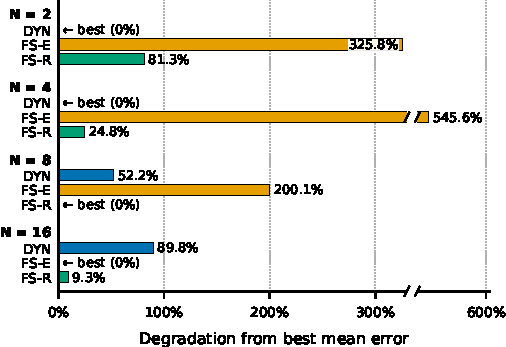
\includegraphics[width=\columnwidth]{./figures/multi_host_ranking.pdf}
	\caption{Average degradation from best mean error vs. $N$ for the heuristics used
	in the three non-dominated strategies.}
        \label{fig:ranking}
\end{figure}


We conclude that \dynamic is more competitive when resources are
scarce, i.e., when closer to the $N{=}1$ case.  As $N$ grows, it is
increasingly important to account for all PEs jointly, which \dynamic does
not do (as it is used independently at each PE).  Consequently, for larger
$N$, greedy heuristics, albeit less sophisticated in terms of local
scheduling decisions, become more competitive than and outperform \dynamic.




\chapter{Optimal Strategies as a Markov Decision Process}
\label{sec:mdp}

Rewriting the recursion as a MDP so it can take into account rescheduling options
including for things like temporal redundancy and reactive rescheduling.

\section{One-PE Formulation}
\label{sec:mdp:onepe}

\noindent{\textbf {State --}}
A state is a pair $(C, n)$, where $n$ is the number of time steps until
the deadline and $C$ is the set of all results reached so far. An element
$(i, x, y) \in C$ denotes an input of $x$ bytes and error level $y$ available
as input to task $T_i$.
Initially $C = \{(1, x_0, y_0)\}$ and $n = H$.  The output error so far is:
$$
y_{\min} (C) = \min\big(\efail, \min_{(M+1, x, y) \in C} y\big).
$$

\noindent{\textbf {Actions --}}
At time zero and after each success or failure, execute any task $T_i$ on
any of its available inputs with any execution mode $j$, given that it
can complete by the deadline and would produce a new output:
\begin{multline*}
A(C, n) = \{ (i, x, y, j) : (i, x, y) \in C, i \leq M, m^i_j \leq n,\\
(i+1, d^i_j(x,y), e^i_j(x,y)) \notin C \}.
\end{multline*}

\noindent{\bf Transitions --}
For action $(i, x, y, j)$:
\begin{compactitem}
\item \textbf{success, with probability $\psuc{m^i_j}$} \\
$(C \cup \{(i+1, d^i_j(x,y), e^i_j(x,y))\}, n - m^i_j)$
\item \textbf{failure during time step $u$, with probability $p_u$}\\ 
$(C, \max(0, n - u - 1 - \lceil R/\deltat \rceil))$.
\end{compactitem}

\noindent{\textbf {Optimal expected error --}}
Let $E(C,n)$ be the optimal expected error from state $(C,n)$.  If
$A(C,n) = \emptyset$ then $E(C,n) = y_{\min}(C)$. Otherwise:
\begin{multline*}
E(C, n) = \min_{(i,x,y,j) \in A(C,n)} \big[\\
\psuc{m^i_j} \times E(C \cup \{(i+1, d^i_j(x,y), e^i_j(x,y))\}, n - m^i_j) + \\
 \sum_{u=0}^{m^i_j - 1} p_u E(C, \max(0, n - u - 1 - \lceil R/\deltat \rceil)) \big].
\end{multline*}
The optimal expected error for the application is $E(\{(1, x_0, y_0)\}, H)$.

\section{Multi-PE Formulation}
\label{sec:mdp:multipe}

\noindent{\textbf {State --}}
A state is a triple $(C, n, \sigma)$. Set $C$ is shared by all PEs, and
$\sigma = (\sigma_1, \ldots, \sigma_N)$ gives the possible statuses of each PE:
\begin{compactitem}
\item available
\item executing task $T_i$ on input $(x,y)$ with mode $j$
\item restarting after a failure
\end{compactitem}

\chapter{Related Work}
\label{sec:related}

%Common techniques for executing applications in the presence of failures
%include replication, checkpointing, and static or dynamic scheduling and
%resource provisioning.  In non-real-time settings, the objective is to
%optimize some performance metric~\cite{10.5555/2811302}.  In real-time
%settings, the objective is to optimize some timeliness metric given
%job/task deadlines~\cite{10.1145/3589950}.

%Examples in real-time
%settings, besides our motivating use case in Chapter~\ref{sec:use-case},
%include Adaptive Bitrate Streaming~\cite{7976298}, in which video
%resolution can be degraded to meet quality-of-service constraints, or the
%use of different precision levels in neural networks to meet
%deadlines~\cite{JIANG2020101775}.

This work targets scenarios in which an application task can implement
different trade-offs between execution time and output error, which is
often termed \emph{approximate computing}~\cite{7348659} and can be
achieved with hardware or software
techniques~\cite{10.1145/3716845,10.1145/3711683}.  Leveraging approximate
computing for real-time applications is a natural idea~\cite{259428,
Leung1995}, which has been explored for various workload and application
models~\cite{10.1002/cpe.4208, 10.1016/j.future.2019.02.019,
STAVRINIDES20101004, 585499, 10.1007/978-3-642-21713-5_20} and remains an
active area of research~\cite{10.1145/3589950}.  The scheduling of
real-time, approximate computing applications, for both aperiodic and
periodic scenarios, has been studied for transient errors, where the
probability of error depends on DVFS levels~\cite{10.1145/2442087.2442094,
10.1007/s11227-021-03764-x}, and for fail-stop failures~\cite{259428,
10.1177/0037549709340729, 10.1109/TC.2003.1183950, 7570524}.


A popular approximate computing model is the \emph{monotone}
model~\cite{259428}: each task consists of a mandatory portion that can
produce output with some error, followed by an optional portion that
incrementally reduces the error and can be interrupted at any time.  This
monotone model is not applicable to the use case that motivates this work,
as the level of approximation of a task must be decided at the onset of its
(re)execution, at which point its execution time and output error level are
fixed, and no usable intermediate output is produced.  Instead of the
monotone model, some works consider that each task comes with a primary
mode (costly, low-error) and an alternate mode (cheap, high-error).  For
instance, the authors in~\cite{10.1109/TC.2003.1183950} propose an approach
in which the primary is always scheduled before the alternate.  In this
work, we consider tasks that can have arbitrary numbers of execution modes.
A natural context in which tasks provide multiple execution modes is when
different DVFS levels lead to different trade-offs between a task's
execution time and the probability that its output is erroneous.
In~\cite{10.1145/2442087.2442094}, the authors focus on periodic tasks with
individual deadlines and seek to minimize energy consumption.
In~\cite{10.1007/s11227-021-03764-x}, the authors have a similar objective
but, like in this work, consider an application with an end-to-end
deadline. In both works, the objective is to minimize energy
consumption while guaranteeing a particular reliability, i.e., bounding the
probability that at least one task output is erroneous.  In contrast,
motivated by the use case in Chapter~\ref{sec:use-case}, in this work some
level of application output error is tolerable and we aim to minimize the
expected error.


The work most closely related to ours is~\cite{10678736}. It considers
deadline-constrained task chains subject to fail-stop failures, where task
execution modes offer different trade-offs between execution time and
output error.  The authors formulate a static resource provisioning
problem: determine optimal choices for the number of application replicas
to execute concurrently, the execution modes for each replica, and the
number of compute resources allocated to each replica, for a given resource
budget.  In contrast, we consider adaptive scheduling decisions throughout
execution, including replication, rollback/recovery, mode changes after
observed failures, reuse of persistent intermediate outputs, and
coordination across PEs. These additional mechanisms require reasoning
about the dynamic execution state rather than making a one-time resource
provisioning decision. To the best of our knowledge, the adaptive
scheduling problem in this work has not been studied previously.



\chapter{Conclusion}
\label{sec:conclusion}

We have studied the problem of scheduling a chain of multi-mode tasks by an
end-to-end deadline in the presence of fail-stop failures. Even a
restricted version of this problem is NP-hard. In the one-PE case, 
dynamic programming makes it possible to precompute optimal scheduling
decisions for a time-discretized version of the problem under a
first-output execution policy. In the multi-PE case, we have proposed
several heuristics.  Using these heuristics in conjunction with temporal
redundancy and reactive rescheduling schemes yields a set of scheduling
strategies.  Simulation results over a large set of application
configurations show which scheduling strategy design choices are sound,
yielding a small set of top-performing strategies with different relative
effectiveness at different platform scales.


Our work can be extended in several ways.  Our temporal redundancy approach
could be extended to re-execute the application from a task $T_i$, $i > 1$,
and/or could be integrated as part of the dynamic program (at the cost of a
much larger state space).  Our experimental results provide a basis upon
which to develop more effective heuristics in the future, e.g., ones that
combine our dynamic programming approach with our greedy heuristics.
Another future work direction is to consider in-situ executions in which
consecutive tasks are merged (to avoid I/O).  Previously proposed task
merging strategies for the purpose of makespan minimization~\cite{6264675}
may be adapted to expected error minimization for multi-mode tasks. In the
multi-PE case, when tasks are parallel programs, an interesting problem is
to find a compromise between having each task use all PEs (as in
Section~\ref{sec:data_parallel}) and each task use a single PE (as in
Chapter~\ref{sec:multihost}).  Finally, a broader future direction is to go
beyond chains and consider more general task graphs.


\bibliographystyle{ieeetr}
\bibliography{references.bib}

\end{document}
